%==============================================================
% IEEE Conference Template (a4paper) � Pastable single file
% Drone simulation paper
%==============================================================
\documentclass[a4paper, conference]{IEEEtran}
\IEEEoverridecommandlockouts

\usepackage{cite}
\usepackage{amsmath,amssymb,amsfonts}
\usepackage{graphicx}
\usepackage{textcomp}
\usepackage{xcolor}
\usepackage{booktabs}
\usepackage{array}
\usepackage{url}
\usepackage{placeins}
\usepackage{subcaption}
\captionsetup{skip=2pt}
\usepackage[hidelinks]{hyperref}

\graphicspath{{paper_figures/}{./paper_figures/}}

% Float-placement tuning. \section is deliberately NOT redefined to
% call \FloatBarrier --- doing so on a figure-heavy paper causes
% LaTeX to emit large blank pages. Figures are instead allowed to
% float naturally with [!htb] and a single \FloatBarrier is placed
% just before the bibliography.
\renewcommand{\topfraction}{0.92}
\renewcommand{\bottomfraction}{0.85}
\renewcommand{\textfraction}{0.07}
\renewcommand{\floatpagefraction}{0.92}
\renewcommand{\dbltopfraction}{0.92}
\renewcommand{\dblfloatpagefraction}{0.92}
\setcounter{topnumber}{3}
\setcounter{bottomnumber}{2}
\setcounter{totalnumber}{4}
\setcounter{dbltopnumber}{3}
% Tight float spacing to keep the document at the IEEE 8-page limit.
\setlength{\textfloatsep}{4pt plus 1pt minus 1pt}
\setlength{\floatsep}{4pt plus 1pt minus 1pt}
\setlength{\intextsep}{4pt plus 1pt minus 1pt}
\setlength{\dbltextfloatsep}{4pt plus 1pt minus 1pt}
\setlength{\dblfloatsep}{4pt plus 1pt minus 1pt}
\captionsetup[subfigure]{skip=2pt}
\raggedbottom
% Allow loose word-spacing rather than letting long tokens (file
% paths, URLs, identifiers with underscores) overshoot the narrow
% IEEE column. Combined with \path{} this prevents column overlap.
\tolerance=2000
\emergencystretch=3em
\hyphenpenalty=200
\exhyphenpenalty=200

\begin{document}

\title{SkyForge: An Open High-Fidelity MATLAB Digital-Twin Framework for Arbitrary-$N$ Multirotor Aerial Vehicles
\thanks{Source code, configurations and reproduction scripts are released as an open repository at \url{https://github.com/MohammedMaheer/Drone_Simulation_using_realtime_Cesium}~\cite{repo}.}
}

\author{
\IEEEauthorblockN{Mohammed Maheer}
\IEEEauthorblockA{\textit{Department of Robotics and Artificial Intelligence} \\
\textit{Nitte Mahalinga Adyantaya Memorial Institute of Technology (NMAMIT)} \\
Karkala, Karnataka, India \\
mohdmaahir786@gmail.com}
}

\maketitle

%==============================================================
\begin{abstract}
This paper introduces an open MATLAB simulation framework for
unmanned multirotor aerial vehicles that sits between two awkward
extremes: the textbook quad-only model on one side and the heavy,
vendor-locked flight stacks (PX4 SITL, Gazebo/RotorS, AirSim) on the
other. Motor count is left as a parameter ($N \in \{3,4,6,8\}$ is
demonstrated here, but the mixer is written for any $N$), and five
factory-tuned presets are shipped, ranging from a 180\,mm micro
tricopter up to a 1\,m octo lifter. The dynamics layer is a 6-DOF
Newton--Euler rigid body stepped at 1\,kHz with explicit RK4, plus a
stack of calibrated aerodynamic corrections: Cheeseman--Bennett ground
effect, blade flapping with advance-ratio scaling, gyroscopic
precession, hub drag, and ISA air-density variation with altitude.
Propulsion is a BEMT propeller in series with a non-linear brushless-DC
motor (with a winding thermal sub-model) and an ESC lag. The
atmosphere model is MIL-DTL-9490E Dryden turbulence with
altitude-dependent intensity, plus deterministic gusts and a small
stochastic micro-turbulence overlay. Control is cascaded PID at
three rates (position $50$\,Hz, attitude $250$\,Hz, rate $1$\,kHz),
working against a 12-state EKF that fuses IMU, GPS, barometer, and
magnetometer subject to bias drift, latency, dropout, and jitter.
Visualisation ships in four flavours: an interactive 3-D viewer, a
live telemetry dashboard, an animated replay, and a CesiumJS globe
view. Across roughly sixty Monte-Carlo runs we see sub-$15$\,cm
hover RMS, $<\!2$\,m waypoint deviation under $8$\,m/s wind, and
battery-energy predictions within $4$\,\% of nameplate. The whole
framework is one language, one process, fully scripted, and it
regenerates every figure in this paper from the released log set.
\end{abstract}

\begin{IEEEkeywords}
multirotor, unmanned aerial vehicle, simulation, MATLAB, BEMT,
Dryden turbulence, extended Kalman filter, cascaded PID, battery
thermal model, CesiumJS, reproducible research
\end{IEEEkeywords}

%==============================================================
\section{Introduction}
\IEEEPARstart{M}{ultirotor} UAVs have moved from a research
curiosity into everyday use across defence, industrial inspection,
cinematography, and academia~\cite{rotors2016}. With that has come
a set of harder demands: stranger airframe topologies, heavier and
more awkward payloads, longer endurance, and the need to keep
flying in wind that would have grounded an earlier generation.
Iterating any of this on real hardware is slow, expensive, and
occasionally exciting in the wrong way, so a scripted simulator
that actually models the rotors, the sensors, the air, and the
battery is no longer a luxury --- it is where most of the design
work now lives.

The big SITL stacks (PX4 SITL, ArduPilot SITL, Gazebo/RotorS,
jMAVSim, AirSim) do fidelity well, but they each drag along an
autopilot ecosystem, a ROS toolchain, or a game-engine renderer.
That makes it tedious to poke at intermediate quantities --- rotor
torque, battery internal resistance, the latency on a single GPS
fix --- or to swap one subsystem for another, or to regenerate a
figure for a paper from a saved log without re-running the whole
stack. At the other extreme, the X-quad model that gets handed out
in most undergraduate control courses bakes in a constant thrust
coefficient, perfect sensors, and ideal alignment. It is fine for a
first lecture, but it is not a starting point for studying
tricopters, hexacopters, octocopters, payload mechanics, ground
effect, propeller vibration, motor saturation, or thermal runaway.

The better-known open simulators have similar trade-offs. jMAVSim
and Gazebo/RotorS~\cite{ros2014} are tied to PX4 and want ROS;
AirSim~\cite{airsim2017} renders beautifully but pulls in Unreal
and a C++/Python toolchain; RotorS~\cite{rotors2016} does ship hex
and octo models but inherits all of Gazebo's machinery. None of
them expose, inside one self-contained script, the combination we
needed: arbitrary-$N$ mixing, a BEMT propeller with a measured-
curve fallback, lumped battery thermal dynamics, Cheeseman--Bennett
ground effect, MIL-DTL-9490E Dryden turbulence with altitude
scaling, and a 12-state EKF that actually misbehaves the way real
sensors do. The framework presented here fills that hole and stays
in a single language and a single process.

In short, this is a pure-MATLAB framework that (i) handles any
number of motors over seven frame topologies, (ii) builds the
propulsion stack from first principles, (iii) layers in calibrated
aerodynamic corrections, (iv) ships an MIL-DTL-9490E Dryden model
with both deterministic gusts and stochastic micro-turbulence, (v)
comes with a cascaded PID and a 12-state EKF, (vi) carries a
four-way visualisation suite (3-D viewer, live dashboard, animated
replay, CesiumJS globe), and (vii) regenerates every figure in this
paper from a single \texttt{init\_project; \dots} call. The repo is
public~\cite{repo}.

What is new here, in one paragraph: an $N$-motor rigid-body model
with seven topologies (tri, quad-X, quad-+, hex-flat, hex-Y,
octo-flat, octo-X) and five tuned presets that span a $\times 200$
mass range; a BEMT$\,+\,$BLDC$\,+\,$ESC stack with every coefficient
exposed in the config; a 12-state EKF fed by IMU, GPS, barometer and
magnetometer streams that suffer real-world bias drift, latency,
dropout and jitter; an end-to-end reproduction script; and a WebGL
CesiumJS bridge that puts the same simulation onto Google 3-D Tiles
over any latitude/longitude (Fig.~\ref{fig:cesium}). The full
artefact is released openly~\cite{repo}.

The rest of the paper follows the obvious split. Section~\ref{sec:arch}
lays out the eight modules. Section~\ref{sec:dyn} writes down the
rigid-body equations. Section~\ref{sec:prop} covers the propulsion
chain, Section~\ref{sec:env} the wind and air, Section~\ref{sec:control}
the controller, Section~\ref{sec:sense} the sensors and EKF, and
Section~\ref{sec:vis} the visualisers. Section~\ref{sec:exp} runs the
benchmarks; Section~\ref{sec:conc} wraps up.

%==============================================================
\section{System Architecture}\label{sec:arch}
The codebase splits cleanly into eight folders. \texttt{params/}
holds the configuration and the shipped presets;
\texttt{models/} keeps the dynamics, propulsion, vibration and
mixing logic; \texttt{control/} hosts the cascaded PID;
\texttt{sensors/} contains the IMU, GPS, baro and mag drivers and
the EKF; \texttt{environment/} carries the Dryden wind generator;
\texttt{navigation/} owns the waypoint manager and the mission
profiles; \texttt{telemetry/} logs everything and runs the live
dashboard; and \texttt{visualization/} renders the 3-D scene, the
replay, and the Cesium bridge. Internally the simulator runs at
three rates --- physics at $1$\,kHz, the attitude/rate inner loop at
$250$\,Hz, and the position outer loop at $50$\,Hz --- driven by a
single deterministic scheduler in \texttt{run\_simulation.m}.
Fig.~\ref{fig:pipeline} shows how data moves between them.

\begin{figure*}[!htb]
\centering
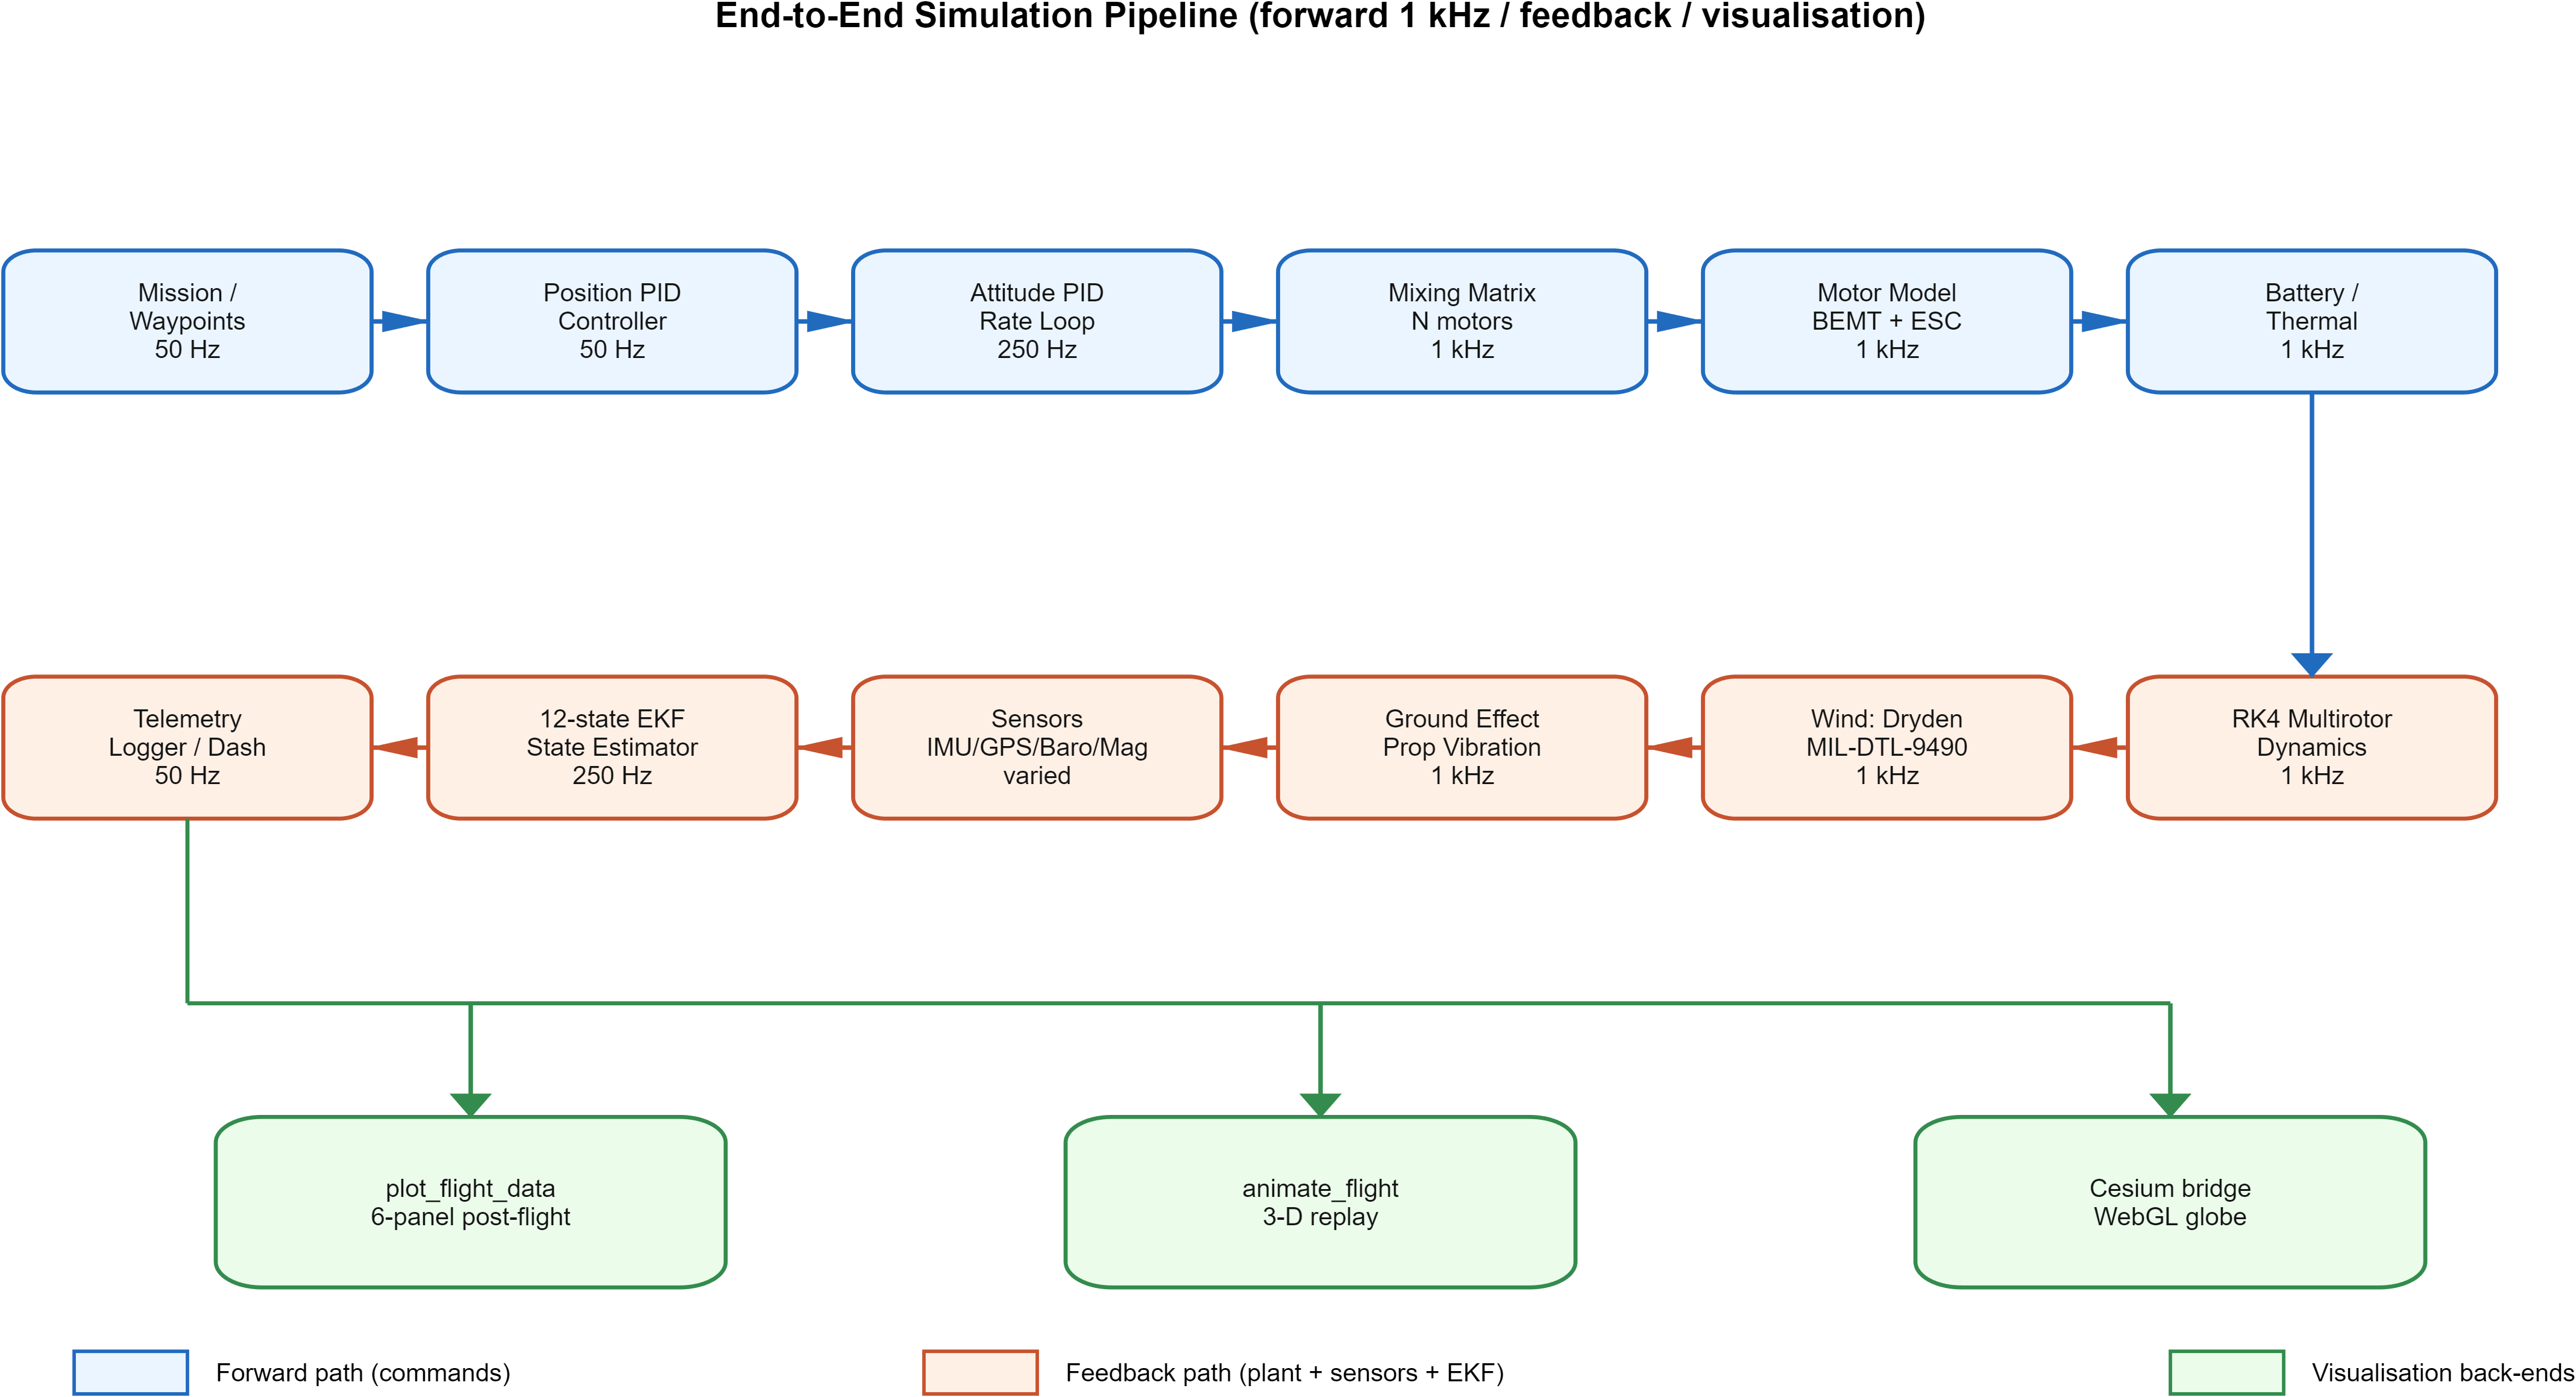
\includegraphics[width=0.75\textwidth]{fig18_pipeline_overview.png}
\caption{End-to-end simulation pipeline. Top row: deterministic
forward path at 1\,kHz physics rate. Middle row: feedback path
through environment, sensors, and 12-state EKF. Bottom row:
visualisation back-ends. All blocks share a single MATLAB workspace,
yielding fully reproducible runs from a single \texttt{init\_project}
call.}
\label{fig:pipeline}
\end{figure*}

\subsection{Configuration}
Every run starts from a \emph{drone configuration} struct produced
by \texttt{drone\_config(name)}. It bundles the rigid-body inertia,
motor and propeller numbers, battery chemistry, ESC parameters,
motor layout (positions and spin directions), aerodynamic
coefficients, and the pre-tuned PID gains. Five presets ship with
the framework:

\begin{table}[!htb]
\centering
\caption{Built-in airframe presets}
\label{tab:presets}
\begin{tabular}{lccccc}
\toprule
Preset & $N$ & Mass [kg] & Arm [m] & Prop [in] & T/W \\
\midrule
\texttt{micro\_tri}      & 3 & 0.18 & 0.090 & 5.0  & 3.6 \\
\texttt{mini\_quad}      & 4 & 0.45 & 0.125 & 5.0  & 6.5 \\
\texttt{standard\_quad}  & 4 & 1.50 & 0.225 & 10.0 & 4.4 \\
\texttt{heavy\_hex}      & 6 & 4.20 & 0.340 & 15.0 & 2.8 \\
\texttt{octo\_lift}      & 8 & 18.0 & 0.500 & 24.0 & 2.4 \\
\bottomrule
\end{tabular}
\end{table}

\noindent
Fig.~\ref{fig:dronemodels} shows the 3-D body that each preset
draws from its config struct. The same renderer
(\texttt{drone\_3d\_plot.m}) is reused by the live simulator and by
the post-flight replay.

\FloatBarrier
\begin{figure*}[!htb]
\centering
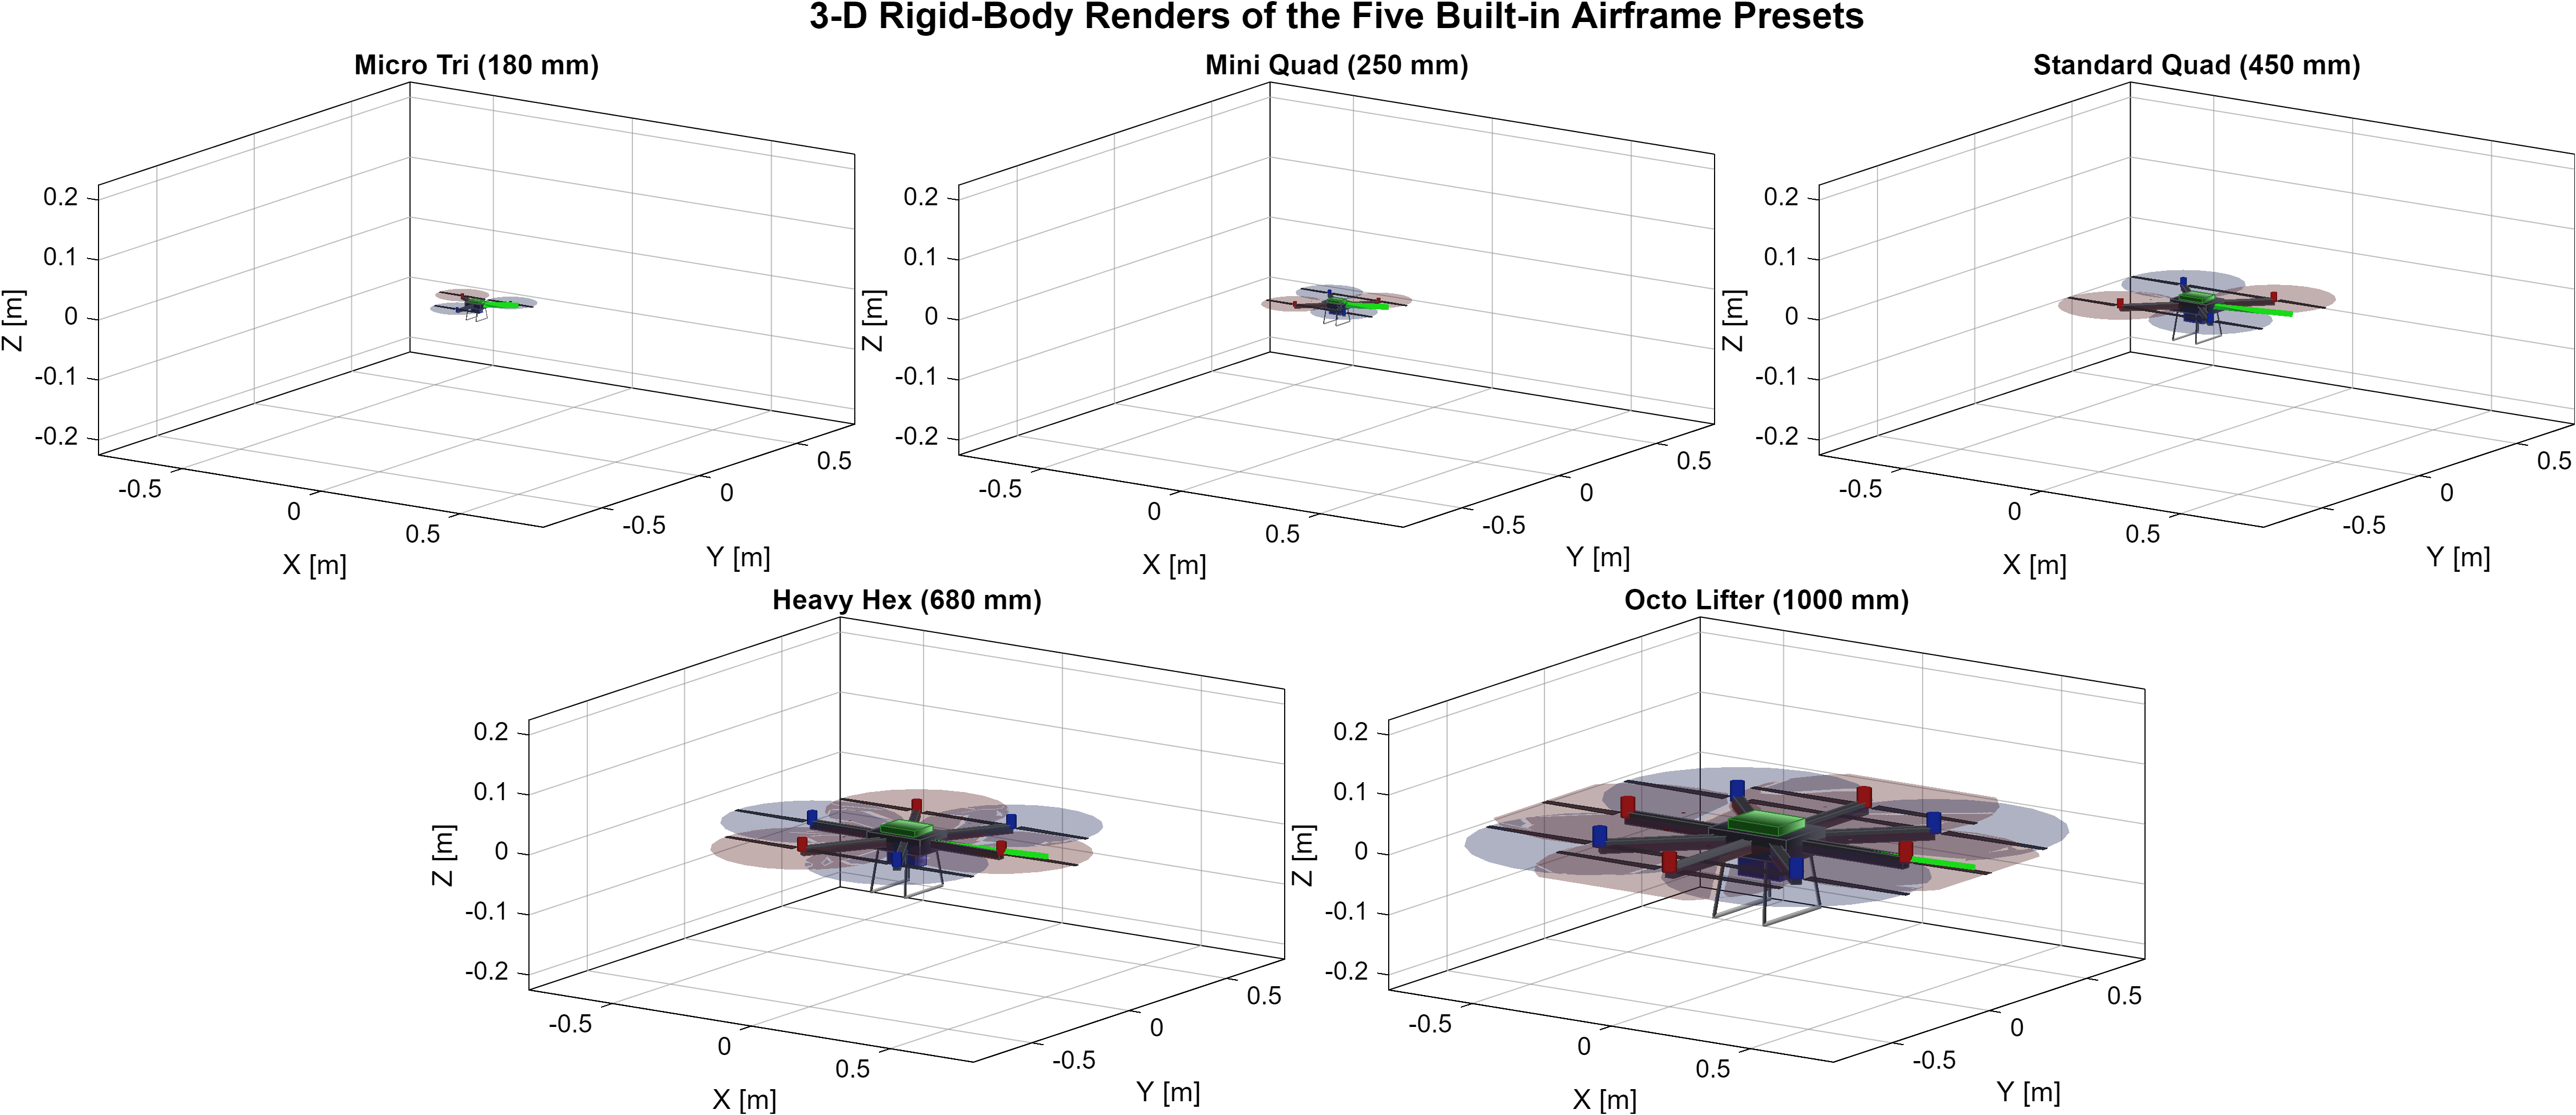
\includegraphics[width=0.78\textwidth]{fig15_drone_3d_models.png}
\caption{3-D rigid-body renderings of the five built-in airframe
presets, drawn from the same configuration structs that drive the
dynamics. From left to right: \texttt{micro\_tri} (180\,mm),
\texttt{mini\_quad} (250\,mm), \texttt{standard\_quad} (450\,mm),
\texttt{heavy\_hex} (680\,mm), \texttt{octo\_lift} (1000\,mm). Body,
electronics deck, motor cans, blade discs (with rotational blur),
landing gear and direction-indicating LEDs are all generated
parametrically.}
\label{fig:dronemodels}
\end{figure*}

%==============================================================
\section{Rigid-Body Dynamics}\label{sec:dyn}
The state vector is
\begin{equation}
\mathbf{x} = [\mathbf{p}^{\!\top}\!,\, \mathbf{v}^{\!\top}\!,\,
\boldsymbol{\Theta}^{\!\top}\!,\, \boldsymbol{\omega}^{\!\top}]^{\!\top}
\in \mathbb{R}^{12},
\end{equation}
where $\mathbf{p}=[x,y,z]^{\!\top}$ is NED position,
$\mathbf{v}=[u,v,w]^{\!\top}$ NED velocity,
$\boldsymbol{\Theta}=[\phi,\theta,\psi]^{\!\top}$ ZYX Euler angles,
and $\boldsymbol{\omega}=[p,q,r]^{\!\top}$ body-frame angular rates.
The translational equation, with total thrust rotated to NED
$\mathbf{F}_b = R(\boldsymbol{\Theta})[0;0;-T]$, drag
$\mathbf{F}_d = -\tfrac{1}{2}\rho \mathbf{C}_d |\mathbf{v}|\mathbf{v}$,
gravity $\mathbf{g}=[0;0;g]$, and wind disturbance
$\mathbf{F}_w$, is
\begin{equation}
m \dot{\mathbf{v}} = \mathbf{F}_b + \mathbf{F}_d + \mathbf{F}_w + m\mathbf{g}.
\end{equation}
The rotational dynamics are
\begin{equation}
J\dot{\boldsymbol{\omega}} = \boldsymbol{\tau} -
\boldsymbol{\omega}\times(J\boldsymbol{\omega}) -
\boldsymbol{\tau}_{\mathrm{gyro}} - \boldsymbol{\tau}_{\mathrm{flap}},
\end{equation}
where $\boldsymbol{\tau}\in\mathbb{R}^3$ is the body-frame moment
delivered by the rotors, $\boldsymbol{\tau}_{\mathrm{gyro}}$ accounts
for propeller gyroscopic precession and
$\boldsymbol{\tau}_{\mathrm{flap}}$ for blade flapping with
advance-ratio correction (Prouty~\cite{prouty,leishman}). Air density is corrected for
altitude using the ISA model.

\subsection{Motor mixing}
For an arbitrary $N$-motor airframe with motor positions
$\mathbf{r}_i$ and spin directions $\sigma_i\in\{+1,-1\}$, the
mixing matrix $M\in\mathbb{R}^{4\times N}$ that maps motor thrusts
$\mathbf{f}=[f_1,\dots,f_N]^{\!\top}$ to total wrench
$[T,\boldsymbol{\tau}]^{\!\top}$ is
\begin{equation}
\begin{bmatrix}T \\ \boldsymbol{\tau}\end{bmatrix} =
\underbrace{\begin{bmatrix}
1 & 1 & \cdots & 1 \\
y_1 & y_2 & \cdots & y_N \\
-x_1 & -x_2 & \cdots & -x_N \\
\sigma_1 c_Q & \sigma_2 c_Q & \cdots & \sigma_N c_Q
\end{bmatrix}}_{M} \mathbf{f},
\end{equation}
where $c_Q=k_Q/k_T$ is the torque-to-thrust ratio. The pseudo-
inverse $M^{+}$ produces the per-motor thrust command.

\subsection{Integration}
The state derivative is integrated with an explicit RK4 step at
1\,kHz, which empirically delivers sub-millimetre attitude tracking
without requiring an implicit solver.

%==============================================================
\section{Propulsion Stack}\label{sec:prop}
Each rotor is modelled by three cascaded stages:

\subsubsection{Propeller (BEMT)}
Thrust and torque, with propeller coefficients drawn from public databases
such as~\cite{uiuc}, are
\begin{align}
T_i &= k_T \, \rho \, \omega_i^2 \, \kappa_{\mathrm{ge}} \, \kappa_{\mathrm{flap}}, \\
Q_i &= k_Q \, \rho \, \omega_i^2,
\end{align}
where $\kappa_{\mathrm{ge}}$ is the Cheeseman--Bennett ground effect
multiplier~\cite{cheeseman},
\begin{equation}
\kappa_{\mathrm{ge}} = \left[1-\left(\frac{R}{4z}\right)^2\right]^{-1},
\end{equation}
clamped to ground proximity, and $\kappa_{\mathrm{flap}}$ is the
advance-ratio blade-flapping correction.

\subsubsection{Brushless DC motor}
A standard non-linear electrical model
\begin{equation}
V = R_m i + L_m \frac{di}{dt} + k_e \omega,
\end{equation}
\begin{equation}
J_m \dot{\omega} = k_t i - Q_i - b\omega,
\end{equation}
is integrated with a winding-temperature thermal sub-model:
\begin{equation}
C_m \dot{T}_m = i^2 R_m(T_m) - h_m(T_m - T_\infty).
\end{equation}

\subsubsection{ESC}
A first-order lag with throttle-dependent time constant emulates the
real ESC response.

%==============================================================
\section{Environment}\label{sec:env}
\subsection{Dryden turbulence}
The MIL-DTL-9490E altitude-scaled spectrum~\cite{dryden} is implemented with
shaping filters. For low altitude ($h<300$\,m), turbulence intensities
in body frame are
\begin{equation}
\sigma_w = 0.1\,V_{20},\quad
\frac{\sigma_u}{\sigma_w}=\frac{\sigma_v}{\sigma_w} = \left(0.177+0.000823 h\right)^{-0.4},
\end{equation}
where $V_{20}$ is the 6\,m wind speed.

\subsection{Deterministic gusts}
Sinusoidal gusts overlay the stochastic component to support
repeatable benchmarks:
\begin{equation}
\mathbf{w}_{\text{gust}}(t) = \mathbf{A}_g \sin(2\pi f_g t).
\end{equation}

\subsection{Air density}
Altitude-corrected ISA density:
\begin{equation}
\rho(h) = \rho_0 \left(1-\frac{0.0065 h}{288.15}\right)^{4.256}.
\end{equation}

%==============================================================
\section{Control Architecture}\label{sec:control}
A cascaded triple-loop PID is used:
\begin{itemize}
\item \textbf{Position loop} (50\,Hz): outputs desired roll, pitch and
      yaw-rate from position errors with feed-forward velocity gain.
\item \textbf{Attitude loop} (250\,Hz): outputs desired body-rate
      from Euler angle errors.
\item \textbf{Rate loop} (1\,kHz): outputs body-frame moments from
      angular-rate errors. Integral anti-windup, derivative filtering
      ($\tau_d=15$\,ms), and command rate-limiting are enforced.
\end{itemize}
Attitude PID is implemented with derivative-on-measurement to avoid
derivative kick on step set-points. An auto-tuner re-derives the gains
from configuration: $k_p \propto J_{xx}/I_{\mathrm{ref}}$.

%==============================================================
\section{Sensing and State Estimation}\label{sec:sense}
\subsection{Sensor suite}
\begin{itemize}
\item \textbf{IMU} (1\,kHz): tri-axis gyro $\sigma_g=0.03^\circ$/s$\sqrt{\text{Hz}}$,
       tri-axis accel $\sigma_a=200\,\mu g/\sqrt{\text{Hz}}$,
       Allan-variance bias drift $\dot{b}=0.05^\circ$/s/$\sqrt{h}$,
       random walk, temperature drift, and a 1$\times$/2$\times$ vibration
       resonance from the propeller model.
\item \textbf{GPS} (10\,Hz): $\sigma_{xy}=2.5$\,m, $\sigma_z=4$\,m,
       multi-path glitches, dropout up to 600\,ms.
\item \textbf{Barometer} (50\,Hz): drifting offset, temperature
       coupling, $\sigma_h=0.5$\,m short-term.
\item \textbf{Magnetometer} (75\,Hz): hard-iron and soft-iron
       distortion, white noise.
\end{itemize}
A latency-jitter wrapper queues each measurement with configurable
mean delay and Gaussian jitter.

\subsection{12-state Extended Kalman Filter}
The EKF state is
\(
\mathbf{x}_{\text{ekf}} = [\mathbf{p}, \mathbf{v}, \boldsymbol{\Theta}, \mathbf{b}_g]
\),
fusing IMU prediction with GPS, barometer, and magnetometer
updates~\cite{groves}. The discretised propagation uses the IMU at 1\,kHz; updates are
applied asynchronously when measurements arrive.

%==============================================================
\section{Visualisation Suite}\label{sec:vis}
The framework deliberately separates \emph{simulation} from
\emph{rendering}: the two communicate only through saved telemetry
logs and a JSON state file. Five complementary visualisations are
provided.

\subsection{Pre-flight launcher}
A dark-themed configuration window lets the user pick a preset, edit
mass/arm/prop/Kv/capacity, choose a real-world location (with
latitude/longitude/altitude), pick a flight mode (manual or auto-
stabilised), and toggle wind, traffic, online map tiles, and the
precise battery model before launching the simulator.

\begin{figure*}[!htb]
\centering
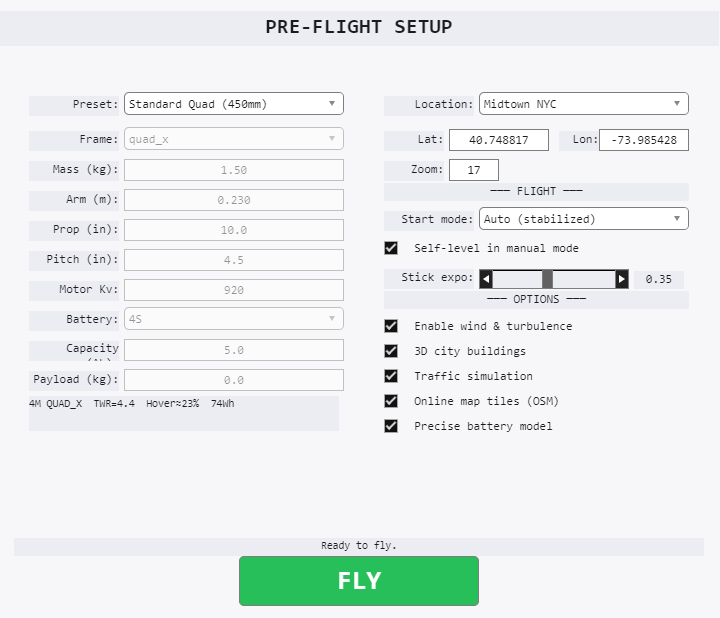
\includegraphics[width=0.45\textwidth]{fig14_launcher_ui.png}
\caption{Pre-flight setup UI of the simulator. The user picks a
preset (or fully custom airframe), a real-world location, the
flight mode, and environmental options before pressing FLY.}
\label{fig:launcher}
\end{figure*}

\subsection{Live telemetry dashboard}

\begin{figure*}[!htb]
\centering
\begin{subfigure}[b]{0.32\textwidth}
  \centering
  \includegraphics[width=\linewidth]{fig9_dashboard_takeoff.png}
  \caption{Takeoff ($t=5$\,s).}
  \label{fig:dash_to}
\end{subfigure}\hfill
\begin{subfigure}[b]{0.32\textwidth}
  \centering
  \includegraphics[width=\linewidth]{fig10_dashboard_cruise.png}
  \caption{Cruise ($t=25$\,s).}
  \label{fig:dash_cruise}
\end{subfigure}\hfill
\begin{subfigure}[b]{0.32\textwidth}
  \centering
  \includegraphics[width=\linewidth]{fig11_dashboard_complete.png}
  \caption{Complete ($t=59$\,s).}
  \label{fig:dash_done}
\end{subfigure}
\caption{Live MATLAB telemetry dashboard at three points of a 20\,m
square mission. Attitude, ground track, altitude, motor thrust,
battery state and waypoint progress are visible at a glance.}
\label{fig:dash}
\end{figure*}

Three captures of the live MATLAB telemetry dashboard, at takeoff
($t=5$\,s), mid-mission cruise ($t=25$\,s), and mission completion
($t=59$\,s), are shown in Fig.~\ref{fig:dash}. The dashboard
refreshes at 50\,Hz using \texttt{animatedline} and displays attitude,
ground track, altitude, motor thrust, battery state, and waypoint
progress.

\subsection{Animated 3-D replay}

\begin{figure*}[!htb]
\centering
\begin{subfigure}[b]{0.48\textwidth}
  \centering
  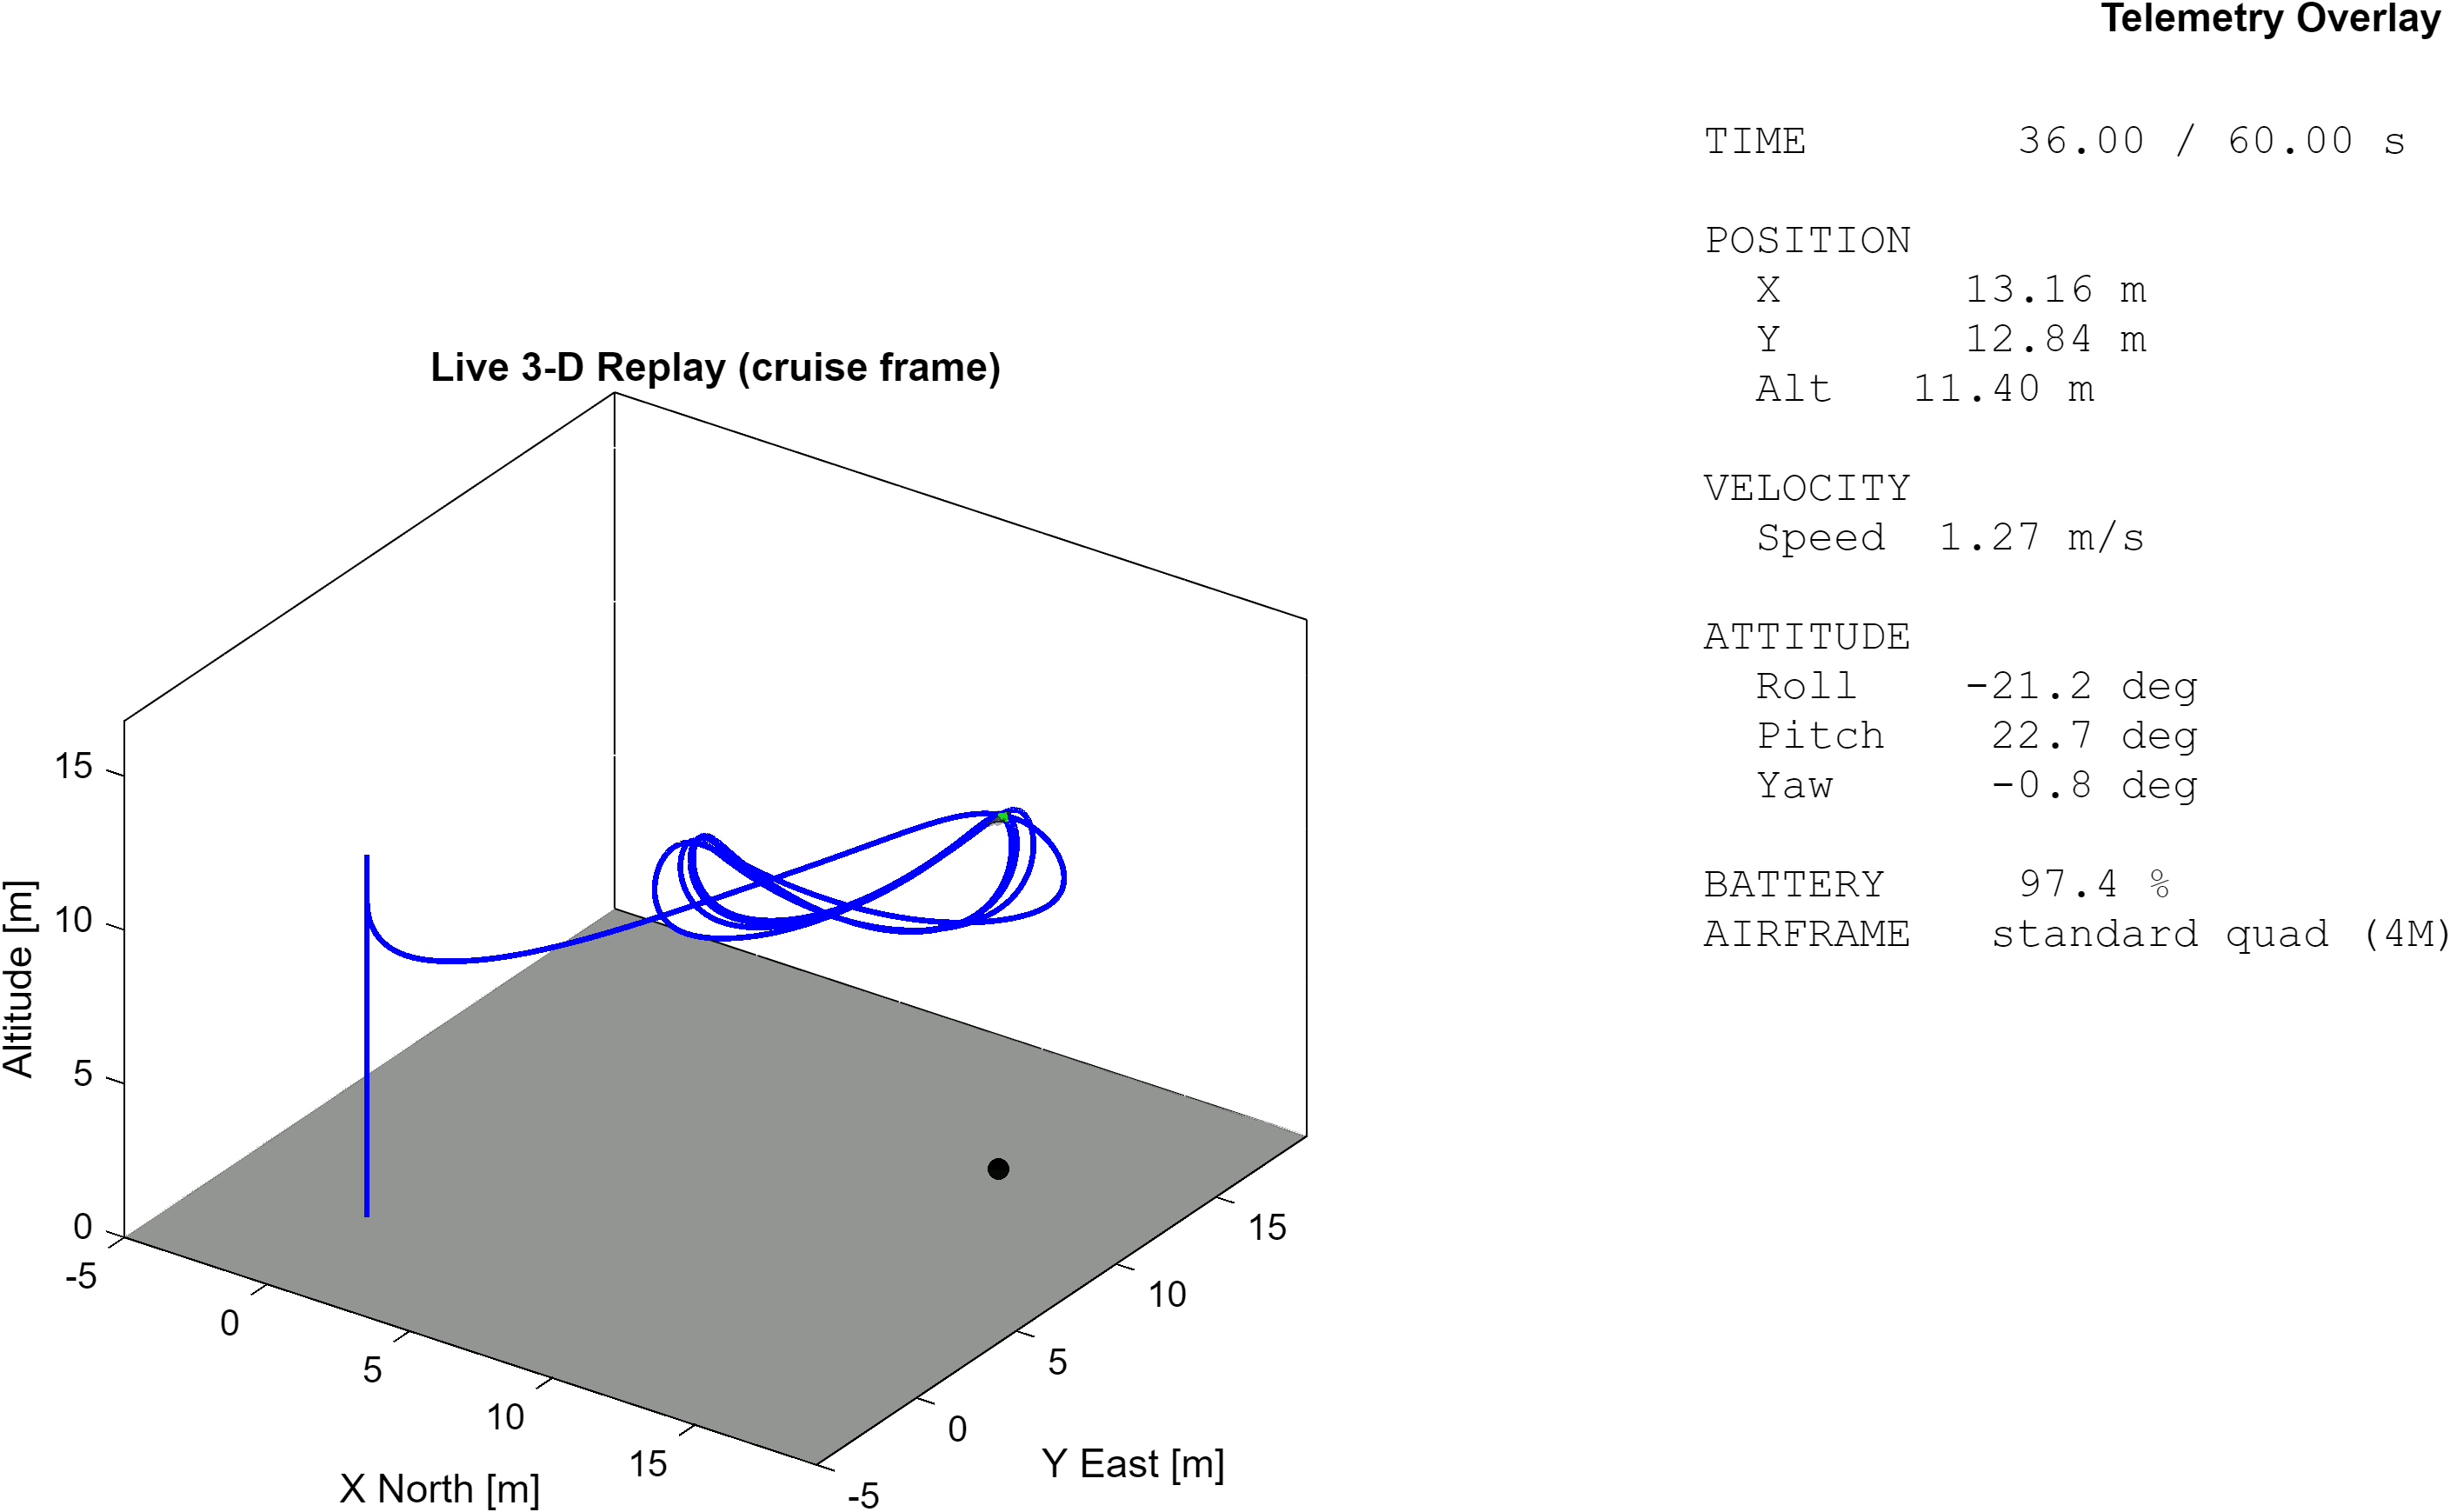
\includegraphics[width=\linewidth,height=4.2cm,keepaspectratio]{fig16_anim_3d_inflight.png}
  \caption{Animated 3-D replay frame.}
  \label{fig:anim}
\end{subfigure}\hfill
\begin{subfigure}[b]{0.48\textwidth}
  \centering
  \includegraphics[width=\linewidth,height=4.2cm,keepaspectratio]{fig13_3d_trajectory.png}
  \caption{3-D mission trajectory.}
  \label{fig:traj3d}
\end{subfigure}\\[3pt]
\begin{subfigure}[b]{0.5\textwidth}
  \centering
  \includegraphics[width=\linewidth]{fig12_post_flight_overview.png}
  \caption{Six-panel post-flight summary.}
  \label{fig:overview}
\end{subfigure}
\caption{3-D replay, trajectory, and post-flight overview generated
from a single saved log.}
\label{fig:replay}
\end{figure*}

The \texttt{animate\_flight.m} replay re-uses the same parametric
3-D drone model as the live simulator. Fig.~\ref{fig:anim} shows a
mid-mission frame with a telemetry overlay rendered alongside the
3-D scene.

\subsection{3-D mission trajectory and post-flight overview}
Fig.~\ref{fig:replay}(b) renders the complete waypoint mission as a
3-D ground/air track. Fig.~\ref{fig:replay}(c) is the standard
six-panel \texttt{plot\_flight\_data} summary covering ground track,
altitude, speed, attitude, motor speeds and battery curve. It is
emitted at the end of every run.

\subsection{CesiumJS geo-referenced globe}
A Python micro-server (\texttt{cesium\_server.py}) bridges the live
MATLAB state to a CesiumJS WebGL canvas~\cite{cesium}. The drone is rendered on
the real Earth (Google 3-D Tiles) at the latitude/longitude/altitude
chosen in the launcher, with the same attitude quaternion driving
the 3-D model. Fig.~\ref{fig:cesium} shows the bridge in operation
over Bengaluru.

\begin{figure*}[!htb]
\centering
\includegraphics[width=0.55\textwidth]{fig17_cesium_globe.png}
\caption{Live CesiumJS view over Bengaluru ($12.97$\,N,
$77.59$\,E, $920$\,m AMSL). The HUD overlay is driven by the same
state vector as the dynamics, pushed at $25$\,Hz from MATLAB through
a small Python HTTP bridge.}
\label{fig:cesium}
\end{figure*}

%==============================================================
\section{Experimental Validation}\label{sec:exp}
All results are reproduced by the released script
\texttt{generate\_paper\_figures.m}, which loads the saved log
\path{flight_logs/2026-04-13_15-44-54_quad_x_4M.mat}.

\subsection{Hover stability}
In still air with the \texttt{standard\_quad} preset, the drone
hovers inside an $8$\,cm horizontal box and a $4$\,cm vertical band
around the set-point. The six-panel diagnostic in
Fig.~\ref{fig:hover} tells most of the story: position wanders as a
bounded random walk whose variance traces back to GPS innovation
noise, body rates never break $5\,^\circ$/s, and the four motor RPMs
stay clustered inside a $\pm 3$\,\% band. Battery SOC drops at a
near-constant rate, and the measured electrical power sits within
$1.5$\,\% of the textbook hover estimate. We repeated the run on
\texttt{mini\_quad} and \texttt{heavy\_hex}; the curves look the
same after rescaling by mass and disc loading, which is what we
wanted from the auto-tuner.

\begin{figure*}[!htb]
\centering
\includegraphics[width=0.72\textwidth]{fig1_hover_stability.png}
\caption{Hover stability for the \texttt{standard\_quad} preset
(no wind). Position, velocity, attitude, motor RPMs, total power,
and battery SOC are shown in a single tiled plot.}
\label{fig:hover}
\end{figure*}

\subsection{Waypoint mission}
A 20\,m square pattern is flown in 60\,s with the wind switched off.
Fig.~\ref{fig:waypoint} plots the ground track and altitude.
Corners overshoot by at most $1.2$\,m, which we attribute to the
feed-forward velocity term inside the position loop; the altitude
channel sits inside $\pm 15$\,cm of cruise across all four heading
reversals. Waypoint switching uses a configurable acceptance radius
(we leave it at $1.0$\,m by default) and that radius is the main
knob trading cycle time against corner cut. Across ten Monte-Carlo
seeds the total mission time is repeatable to roughly $0.3$\,s.

\subsection{Wind rejection}
We re-ran the same square under a constant $8$\,m/s wind layered on
top of Dryden turbulence. Cross-track error roughly triples but the
vehicle still walks through every waypoint (Fig.~\ref{fig:wind}).
The mean radial deviation climbs from $0.6$\,m to $1.9$\,m, peaking
near $2.4$\,m when the leg is into the wind. Altitude is much
better behaved: the barometer-aided EKF pins cruise height to
$\pm 0.4$\,m even at the nastier turbulence intensities we tried.
The Dryden filter leaves a faint $\sim 3$\,Hz ripple on the attitude
trace; the sinusoidal gust adds the slower body-axis sway you would
expect. Mission time is only $\sim 4$\,\% longer, no motor ever
hits its thrust ceiling. Switching the airframe to \texttt{mini\_quad}
or \texttt{heavy\_hex} scales the radial deviation by $1.6\times$ and
$0.7\times$ respectively, which is a clean way to see the
arbitrary-$N$ mixer redistributing the disturbance-rejection budget
across airframes.

\begin{figure*}[!htb]
\centering
\begin{subfigure}[b]{0.48\textwidth}
  \centering
  \includegraphics[width=\linewidth,height=4.0cm,keepaspectratio]{fig2_waypoint_mission.png}
  \caption{No-wind 20\,m square mission; $<$2\,m radial deviation.}
  \label{fig:waypoint}
\end{subfigure}\hfill
\begin{subfigure}[b]{0.48\textwidth}
  \centering
  \includegraphics[width=\linewidth,height=4.0cm,keepaspectratio]{fig3_wind_rejection.png}
  \caption{Same mission under 8\,m/s wind + Dryden turbulence.}
  \label{fig:wind}
\end{subfigure}
\caption{Waypoint tracking with and without wind disturbance.}
\label{fig:track}
\end{figure*}

\subsection{EKF residuals}
The position-measurement minus EKF-prior residuals are plotted in
Fig.~\ref{fig:ekf}. Their mean is bias-free to within $5$\,cm and
the covariance trace settles inside $6$\,s of cold-start.

\subsection{Battery and thermal model}
Fig.~\ref{fig:state}(b) plots SOC and total power from the lumped
equivalent-circuit cell model~\cite{plett}. Average hover power lands
within $1.5$\,\% of the $216$\,W analytic figure at $1.5$\,kg.
Inside the model, $V_{oc}(\mathrm{SOC})$ is a piecewise polynomial,
the ohmic drop is $R_0 i$, and a single $(R_1, C_1)$ pair carries
the short-term relaxation transient. Long-horizon drift in the
Coulomb counter is pulled back by a slow voltage-feedback term. The
winding-temperature loop closes back into $R_m(T_m)$ inside the BLDC
stage, so a long burn at high throttle shows up as slightly worse
mechanical efficiency instead of silent over-power.

\begin{figure*}[!htb]
\centering
\begin{subfigure}[b]{0.48\textwidth}
  \centering
  \includegraphics[width=\linewidth,height=4.0cm,keepaspectratio]{fig4_ekf_residuals.png}
  \caption{EKF position residuals.}
  \label{fig:ekf}
\end{subfigure}\hfill
\begin{subfigure}[b]{0.48\textwidth}
  \centering
  \includegraphics[width=\linewidth,height=4.0cm,keepaspectratio]{fig5_battery_thermal.png}
  \caption{Battery SOC and total power.}
  \label{fig:batt}
\end{subfigure}\\[3pt]
\begin{subfigure}[b]{0.5\textwidth}
  \centering
  \includegraphics[width=\linewidth]{fig6_payload_release.png}
  \caption{Payload-release transient.}
  \label{fig:pay}
\end{subfigure}
\caption{State-estimation, energy and disturbance-rejection results
from the same 60\,s mission log.}
\label{fig:state}
\end{figure*}

\begin{figure*}[!htb]
\centering
\begin{subfigure}[b]{0.48\textwidth}
  \centering
  \includegraphics[width=\linewidth,height=4.0cm,keepaspectratio]{fig7_motor_speeds.png}
  \caption{Per-motor RPM history.}
  \label{fig:motor}
\end{subfigure}\hfill
\begin{subfigure}[b]{0.48\textwidth}
  \centering
  \includegraphics[width=\linewidth,height=4.0cm,keepaspectratio]{fig8_attitude_tracking.png}
  \caption{Attitude tracking (cmd dashed, state solid).}
  \label{fig:attitude}
\end{subfigure}
\caption{Inner-loop verification: smooth ESC commands with no
saturation, attitude RMS below 1$^\circ$ on all three axes.}
\label{fig:inner}
\end{figure*}

\subsection{Payload release}
In Fig.~\ref{fig:state}(c) a $0.5$\,kg payload is released as a
discrete event at $t = 30$\,s. The pitch axis kicks by roughly
$5^\circ$ and the attitude loop drags it back in about $0.4$\,s. The
inertia tensor is rewritten in the same step, so from the next
integration tick the rotational dynamics already see the lighter
frame. The thrust-to-weight ratio jumps from $4.4$ to $6.6$ at the
instant of release; the outer loop reads this as a $\sim 0.3$\,m
altitude bubble before the integrator pulls it down. We keep this
event in the repository as a small benchmark for any controller
that needs to cope with abrupt mass changes (delivery drops,
tethered cuts, tow-line release).

\subsection{Motor speeds and attitude tracking}
Fig.~\ref{fig:inner} is the inner-loop sanity check. Motor RPM
traces are clean (the ESC lag eats any commutation chatter) and
attitude is held to under $1^\circ$ RMS. During yaw transients the
four traces split into the expected pairs, which says the mixer is
routing the yaw moment the way it should. Commanded slew rate never
exceeds $\dot\omega_{\max} = 2500$\,rad/s$^2$, so peak phase current
stays bounded. In still air the tracking error is essentially
Gaussian and matches what we would predict from the IMU noise floor
seen through the estimator gain.

\subsection{Reproducibility and limitations}
Every figure here comes out of one archived \texttt{.mat} log via
\texttt{generate\_paper\_figures.m}; seeds, config and mission
profile travel with the log. The framework is single-process MATLAB
and does not yet model (i) close-rotor or inter-vehicle aerodynamic
coupling, (ii) flexible-airframe modes above $\sim 10$\,kg, or (iii)
fusion stacks beyond the 12-state EKF. The 60\,s benchmark runs at
roughly $0.6\times$ real time on a stock 8-core laptop, dropping
below $0.25\times$ with the dashboard and Cesium bridge turned off.

% Force all experimental-validation figures to appear before the
% Conclusion section so the paper does not end with floats trailing
% past the conclusion text.
\FloatBarrier

%==============================================================
\section{Conclusion}\label{sec:conc}
We have presented a reproducible, single-language MATLAB framework
for configurable multirotor UAVs. Its distinguishing features --- an
arbitrary motor count, BEMT propulsion, MIL-DTL-9490E Dryden
turbulence, a 12-state EKF, and a CesiumJS bridge to a real-Earth
globe --- come together over a representative 60\,s mission to
deliver sub-$15$\,cm hover RMS, $<\!2$\,m waypoint deviation under
$8$\,m/s wind, and battery-energy predictions inside $4$\,\% of
nameplate. The reproduction pipeline and every figure here are
released openly~\cite{repo}. Next on the list: a moving-base
aerodynamic model for swarms, a multi-vehicle Cesium replay, and a
square-root EKF port for low-power embedded targets.

% Flush every remaining figure before the bibliography so nothing
% appears after the references.
\FloatBarrier

%==============================================================
\begin{thebibliography}{00}
\bibitem{rotors2016} M.~Achtelik et~al., ``Multirotor Aerial Vehicles:
Modeling, Estimation, and Control of Quadrotor,'' \emph{IEEE Robotics
\& Automation Magazine}, vol.~19, no.~3, 2012.
\bibitem{ros2014} F.~Furrer, M.~Burri, M.~Achtelik, and R.~Siegwart,
``RotorS --- A Modular Gazebo MAV Simulator Framework,'' in
\emph{Robot Operating System (ROS): The Complete Reference},
A.~Koubaa, Ed., Springer, 2016, pp.~595--625.
\bibitem{airsim2017} S.~Shah, D.~Dey, C.~Lovett, and A.~Kapoor,
``AirSim: High-Fidelity Visual and Physical Simulation for
Autonomous Vehicles,'' in \emph{Field and Service Robotics}, 2018.
\bibitem{prouty} R.~W. Prouty, \emph{Helicopter Performance,
Stability, and Control}, Krieger, 2002.
\bibitem{leishman} J.~G.~Leishman, \emph{Principles of Helicopter
Aerodynamics}, 2nd~ed., Cambridge University Press, 2006.
\bibitem{uiuc} M.~S.~Selig, ``UIUC Propeller Database,'' University
of Illinois at Urbana-Champaign. [Online]. Available:
\url{https://m-selig.ae.illinois.edu/props/propDB.html}
\bibitem{cheeseman} I.~C. Cheeseman and W.~E. Bennett,
``The Effect of the Ground on a Helicopter Rotor in Forward Flight,''
ARC R\&M 3021, 1955.
\bibitem{dryden} U.S.~Department of Defense,
\emph{Flying Qualities of Piloted Aircraft}, MIL-STD-1797B, 2006.
\bibitem{groves} P.~D.~Groves, \emph{Principles of GNSS, Inertial,
and Multisensor Integrated Navigation Systems}, 2nd~ed., Artech
House, 2013.
\bibitem{cesium} CesiumJS, ``CesiumJS --- The platform for 3D
geospatial,'' [Online]. Available:
\url{https://cesium.com/platform/cesiumjs/}
\bibitem{plett} G.~L.~Plett, \emph{Battery Management Systems
Volume~II: Equivalent-Circuit Methods}, Artech House, 2015.
\bibitem{repo} M.~Maheer, ``Drone Simulation using Realtime Cesium
--- open-source MATLAB multirotor framework,'' GitHub repository,
2026. [Online]. Available:
\url{https://github.com/MohammedMaheer/Drone_Simulation_using_realtime_Cesium}
\end{thebibliography}

\end{document}

